\chapter{Introduction}\label{ch:intro}

\def \path {intro}
\def \imgpath {\path/images}

It has long been the goal of computer vision researchers to be able to develop
systems that can reliably recognize objects in a scene. Achieving this unlocks a huge
range of applications that can benefit society as a whole. From fully
autonomous vehicles, to automatic labelling of uploaded videos/images for searching,
or facial recognition for identification and security, the uses are far
reaching and extremely valuable. The challenge does not lie in finding the
right application, but in the difficulty of training a computer to \emph{see}.

There are nuisance variables such as changes in
lighting condition, changes in viewpoint and background clutter that do not
affect the scene but drastically change the pixel representation of it. 
Humans, even at early stages of their lives, have little difficulty filtering
these out and extracting the necessary amount of information from a scene. So
to design a robust system, it makes sense to design it off how \emph{our}
brains see. 

Unfortunately, vision is a particularly complex system to understand. It has
more to it than the simply collecting photons in the eye.
An excerpt from a recent Neurology paper \cite{raichle_two_2010} sums up the problem
well:

\begin{quotation}
It might surprise some to learn that visual information is significantly
degraded as it passes from the eye to the visual cortex. Thus, of the unlimited
information available from the environment, only about $10^{10}$ bits/sec are
deposited in the retina \ldots\ only $\sim 6\times 10^6$
bits/sec leave the retina and only $10^4$ make it to layer IV of V1
\cite{anderson_directed_2005,tor_norretranders_user_1998}. These data
clearly leave the impression that visual cortex receives an impoverished
representation of the world \ldots\ it should be noted that estimates of the
bandwidth of conscious awareness itself (i.e.,\ what we `see') are in the range
of 100 bits/sec or less\cite{anderson_directed_2005,
tor_norretranders_user_1998}.
\end{quotation}

Current digital cameras somewhat act as a combination of the first and second
stage of this system, collecting photons in photosensitive sensors and then
converting this to an image on the order of magnitude of $10^6$ pixels (slightly
larger but comparable to the $10^6$ bits/sec travelling through the optic
nerve).

If we are to build effective vision systems, it makes sense to emulate this
compression of information.
The question now stands before us --- what information is kept on entry to the V1 cortex?
Hubel and Wiesel revolutionized our understanding of the V1 cortex in the 50s and 60s by 
studying cats \cite{hubel_receptive_1959, hubel_receptive_1962}, macaques and spider 
monkeys \cite{hubel_receptive_1968}. They found that neurons in the V1 cortex fired
most strongly when edges of a particular (i.e.,\ neuron-dependent) orientation
were presented to the animal, so long as the edge was inside the receptive field of
this neuron.
Continued work on their experiments by Blakemore and Cooper
\cite{blakemore_development_1970} showed that these early layers of perception
are in fact \emph{learned}. Their experiments kept kittens in darkness and exposed
them a few hours a day to only horizontal or vertical lines. After five months, they were
taken into natural environments and their reactions were monitored. The two groups of cats
would only play with rods that matched the orientation of their environment.
% A figure of the the frequency response of the photoreceptor cells in our eyes
% to different wavelengths of light.
% \begin{figure}
  % \begin{center}
      % 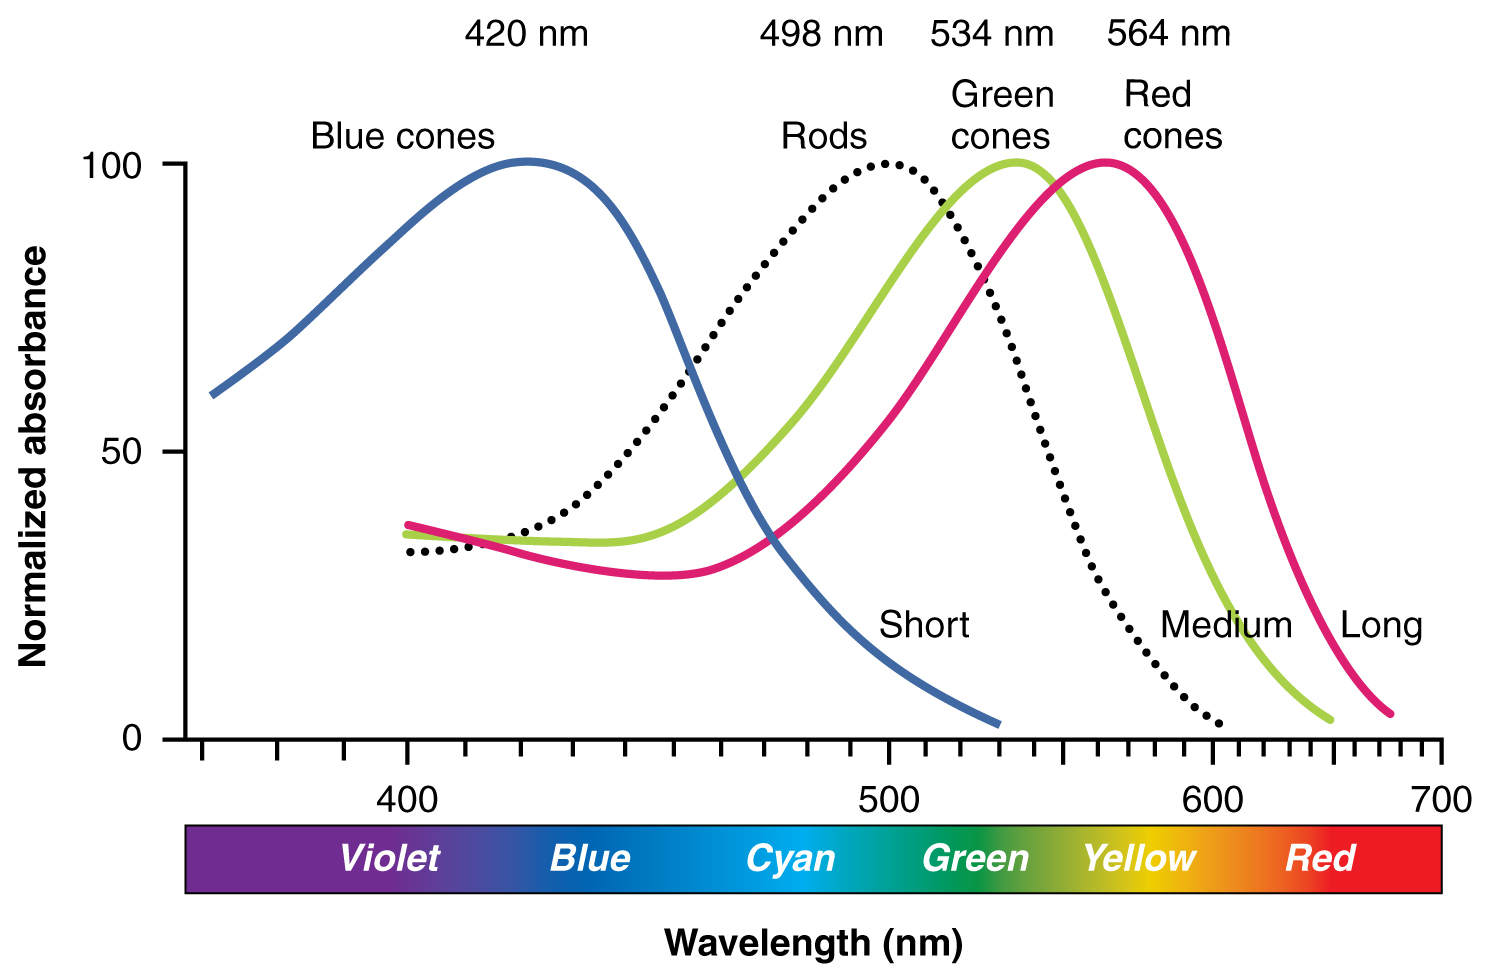
\includegraphics[width=10cm]{\imgpath/colour_sensitivity.jpg}
      % \mycaption{Frequency sensitivity of photoreceptors in they eye}
              % {Wavelength responsiveness of the different photoreceptors in the
               % eye. S, M, and L are short, medium, and long cones, compared to
               % R --- rods. Taken from~\cite{bowmaker_visual_1980}}
  % \end{center}
% \end{figure}

\section{Convolutional Neural Networks}
\begin{figure}
  \centering
    % \includegraphics[width=\textwidth]{\imgpath/dtcwt_gain}
    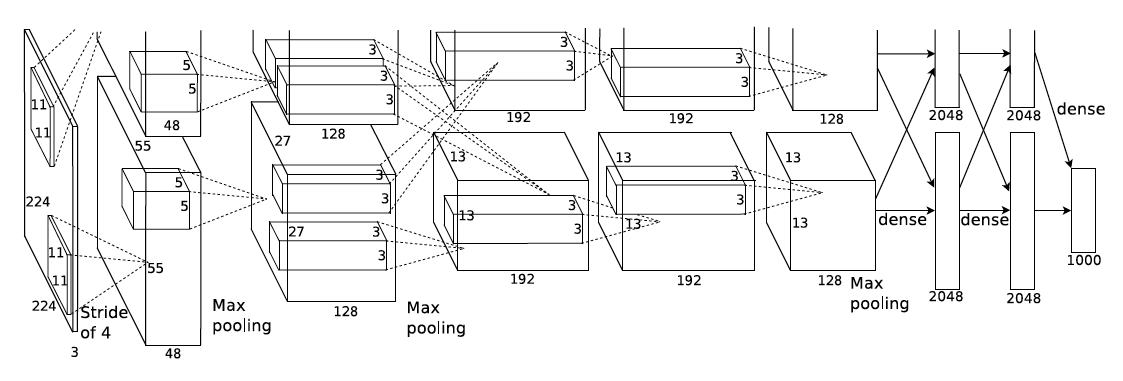
\includegraphics[width=\textwidth]{\imgpath/alexnet.png}
    \mycaption{Convolutional Architecture example}{The previous layer's activations are
    combined with a learned convolutional filter.
    Note that while the activation maps are 3D arrays, the convolution is only
    a 2D operation. This means the filters have the same number of channels as
    the input and produce only one output channel. Multiple channels are made by
    convolving with multiple filters. Not shown here are the nonlinearities that
    happen in between convolution operations. Image taken from \cite{krizhevsky_imagenet_2012}}.
    \label{fig:ch1:cnn_arch}
  \end{figure}
The current state of the art in image understanding sysems are 
Convolutional Neural Networks (CNNs). These are a learned model that
stacks many convolutional filters on top of each other separated by
nonlinearities. 
They are seemingly inspired by the visual cortex in the way that they are
hierarchically connected, progressively compressing the information into a
richer representation. 

\autoref{fig:ch1:cnn_arch} shows an example 
architecture for the famous AlexNet \cite{krizhevsky_imagenet_2012}. Inputs are resized to a
manageable size, in this case $224\x 224$ pixels. Then multiple convolutional
filters of size $11\x 11$ are convolved over this input to give $96$ output
\emph{channels} (or \emph{activation maps}). In the figure, these are split onto two 
graphics cards or GPUs for memory purposes. These are then passed through a
a pointwise nonlinear function, or a \emph{nonlinearity}.
The activations are then pooled (a form of downsampling) and convolved with more
filters to give $256$ new channels at the second stage. This is repeated 3 more
times until the $13\x 13$ output with $256$ channels is unravelled and passed
through a fully connected neural network to classify the image as one of $1000$
possible classes.
  
CNNs have garnered lots of attention since 2012 when the previously mentioned AlexNet
nearly halved the top-5 classification error rate (from $26\%$ to $16\%$) 
on the ImageNet Large Scale Visual Recognition Competition (ILSVRC)
\cite{russakovsky_imagenet_2014}\footnote{The previous state of
the art classifiers had been built by combining keypoint extractors like 
SIFT\cite{lowe_distinctive_2004} and HOG\cite{dalal_histograms_2005} with
classifiers such as Support Vector Machines\cite{cortes_support-vector_1995} and
Fisher Vectors\cite{sanchez_image_2013}, for example \cite{sanchez_high-dimensional_2011}.}.
In the years since then, their complexity has grown significantly. AlexNet had
only 5 conovlutional layers, whereas the 2015 ILSVRC winner ResNet \cite{he_deep_2016}
achieved 3.57\% top-5 error with 151 convolutional layers (and had some
experiments with 1000 layer networks).

\section{Issues with CNNs}\label{sec:ch1:motivation}
\begin{figure}
  \centering
  \subfloat[conv1 filters]{
  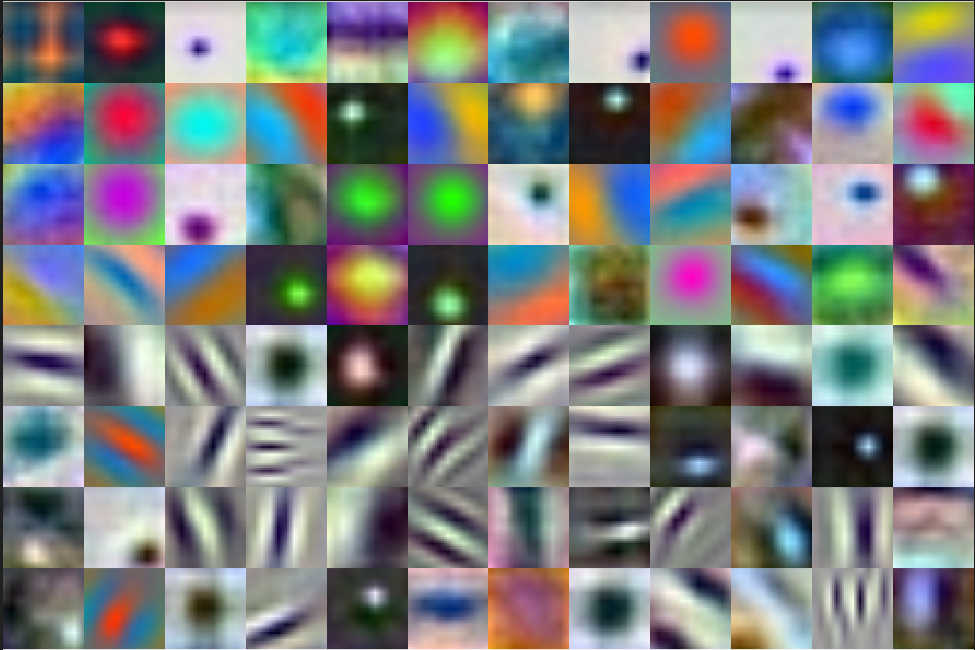
\includegraphics[width=0.6\textwidth]{\imgpath/alexfilters.png}
  \label{fig:ch1:alex_filt}
  }\\
  \subfloat[conv1 activations]{
  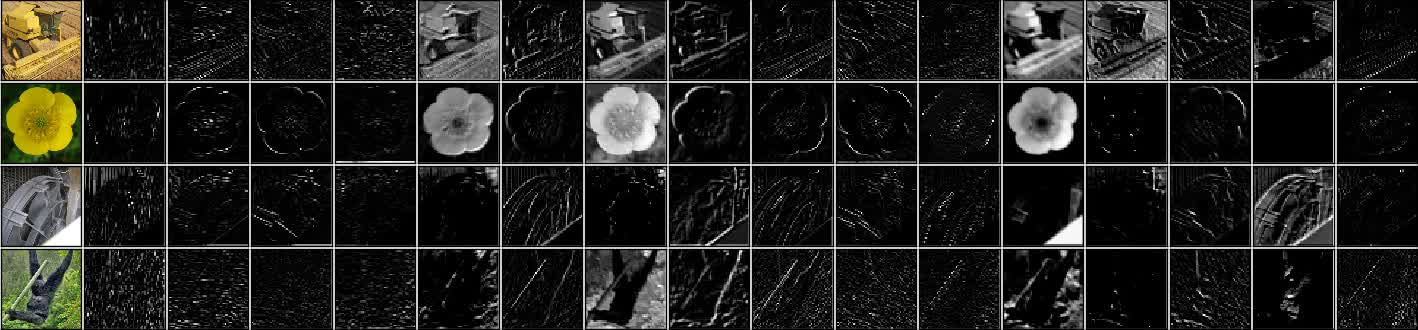
\includegraphics[width=\textwidth]{\imgpath/out1.jpg}
  \label{fig:ch1:alex_conv1}
  }\\
  \subfloat[conv2 activations]{
  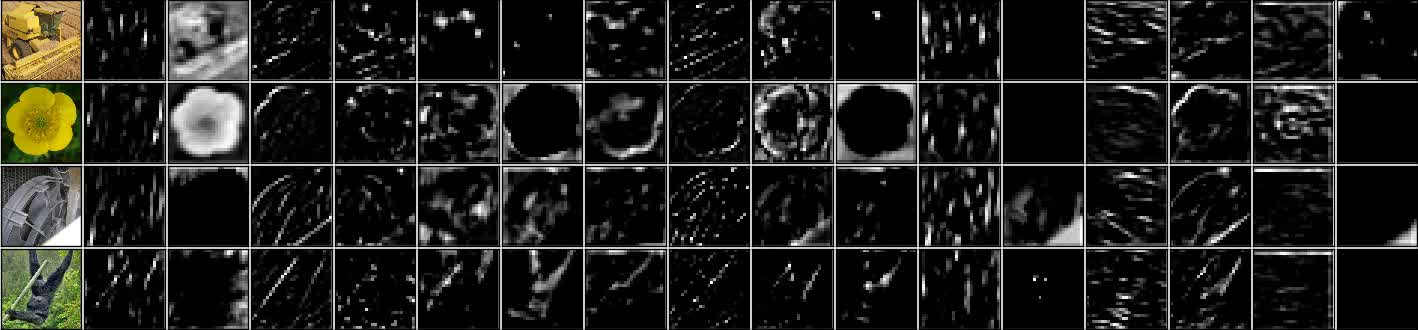
\includegraphics[width=\textwidth]{\imgpath/out2.jpg}
  \label{fig:ch1:alex_conv2}
  }\\
  \subfloat[conv3 activations]{
  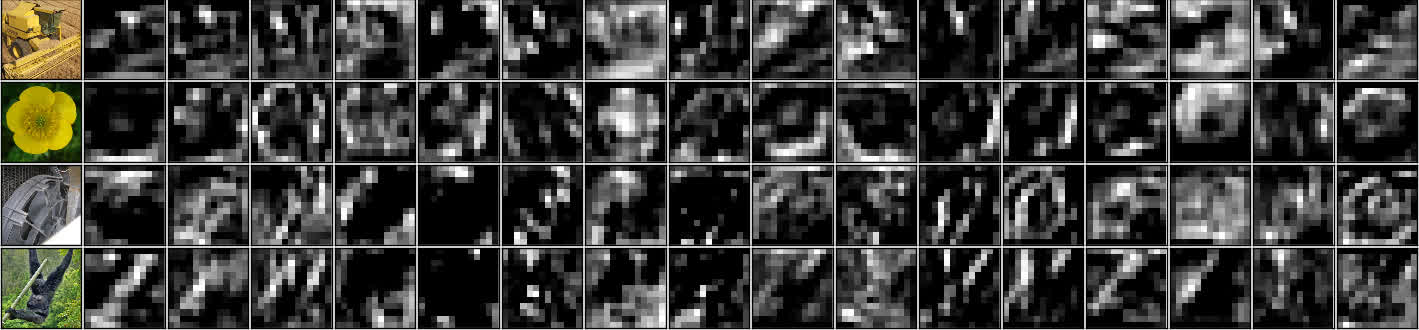
\includegraphics[width=\textwidth]{\imgpath/out3.jpg}
  \label{fig:ch1:alex_conv3}
  }
  \mycaption{Example first layer filters and the first three
  layer's outputs}{\subref{fig:ch1:alex_filt} The $11\x 11$ filters for the
  first stage of AlexNet. Of the 96 filters, 48 were learned on one GPU and
  another 48 on another GPU. Interestingly, one GPU has learned mostly
  lowpass/colour filters and the other has learned oriented bandpass
  filters. \subref{fig:ch1:alex_conv1} - \subref{fig:ch1:alex_conv3} Randomly
  chosen activations from the output of the first, second and third convolutional 
  layers of AlexNet (see \autoref{fig:ch1:cnn_arch}) with negative values set to 0. 
  Filters and activation images taken from supplementary material of
    \cite{krizhevsky_imagenet_2012}.}
  \label{fig:ch1:alexnet_filters}
\end{figure}
Despite their success, they are often criticized for being \emph{black box}
methods. You can view the first layer of filters
quite easily (see \autoref{fig:ch1:alex_filt}) as they exist in RGB
space, but beyond that things get trickier as the filters have a third, \emph{depth}
dimension typically much larger than its two spatial dimensions. Additionally,
it is not clear what the input channels themselves correspond to. For illustration
purposes, we have also shown some example activations from the first three
convolutional layers for AlexNet in
\autoref{fig:ch1:alexnet_filters}\subref{fig:ch1:alex_conv1}-\subref{fig:ch1:alex_conv3}\footnote{These activations are
taken after a specific nonlinearity that sets negative values to 0, hence the
large black regions.}. We can see in \autoref{fig:ch1:alex_conv1} that
in the conv1 activations, some of the first layer channels are responding to
edges or colour information, but as we go deeper to conv2 and conv3, it becomes
less and less clear what each activation is responding to.

Aside from their lack of interpretability, it takes a long time and a lot of
effort to train state of the art CNNs. Typical networks that have won ILSVRC
since 2012 have had roughly 100 million parameters and take up to a week to train. This 
is optimistic and assumes that you already know the necessary optimization or
architecture hyperparameters, which you often have to find out by trial and error. 
In a conversation the author had with Yann LeCun, the attributed father of
CNNs, at a Computer Vision Summer School (ICVSS), LeCun highlighted this problem
himself:
\begin{quote}
  There are certain recipes (for building CNNs) that work and certain recipes
  that don't, and we don't know why.
\end{quote}

Considering the recent success of CNNs, it is becoming more and more
important to understand \emph{how} and \emph{what} a network learns, which
has contributed to it making its classification or regression choice.
Without this information, the use of these incredibly powerful tools could be
restricted to research and proprietary applications.

\section{An Interesting Result - The Learned Wavelet Transform}
The structure of convolutional layers is fairly crude in terms of signal
processing - arbitrary taps of an FIR filter are learned typically via gradient
descent to minimize either a mean-squared error or cross entropy loss. It is perhaps surprising
and motivating then that the filters we saw earlier learned by the first layer of a CNN
(\autoref{fig:ch1:alexnet_filters}) look like oriented wavelets. 
From a biological point of view this makes sense, as it matches the earlier
mentioned results by Hubel and Wiesel. From a signal processing point of view
this also makes sense, as the wavelet transform is a powerful and stable way to
split up an image into areas of the frequency domain.  
However, there was no prior placed on the filters to make them have 
this similarity to wavelets. There were no constraints on vanishing
moments\cite{daubechies_ten_1992} or smoothness, or even for the `conv1' activations
to be sparse; the only constraint they had was an $\ell_2$ penalty to avoid large
filter taps.


\section{Project Motivation}
This leads us to ask a motivating question:

\begin{quote}
  Is it possible to learn convolutional filters as 
  combinations of basis functions rather than individual filter taps?
\end{quote}

However in achieving this, it is important to find ways to have an adequate
richness to filtering while reducing the number of parameters needed to specify
this. We want to contract the space of learning to a subspace or manifold that 
is more useful. In much the same way, the convolutional layer in a CNN is a restricted
version of a fully connected layer in a multi-layer perceptron, yet adding this
restriction allowed us to train more powerful networks. 

The intuition that we explore in this thesis is that \emph{complex wavelets} are the
right basis functions for convolutional filtering in CNNs. We have already seen in the
previous section that they would do well in replacing the first layer of a CNN,
but can they be used at deeper layers? Their well understood and
well defined behaviour would help us to answer the above \emph{how} and \emph{why}
questions. Additionally, they allow us to enforce a certain amount of smoothness and near
orthogonality; smoothness is important to avoid sensitivity to adversarial or
spoofing attacks \cite{szegedy_intriguing_2013} and near orthogonality
allows you to cover a large space with fewer coefficients.

But first we must find out \emph{if} it is possible to get the same or near the same
performance by using wavelets as the building blocks for CNNs, and this is the
core goal of this thesis. 

\section{ScatterNets}
To explore this intuition, we begin by looking at one of the most
popular current uses of wavelets in image recognition tasks, the
Scattering Transform. 
The Scattering Transform, or the \emph{ScatterNet}, was introduced in \cite{mallat_group_2012,
bruna_invariant_2013} at the same time as AlexNet. It is a non black box
network that can be thought of as a restricted complex valued CNN
\cite{bruna_mathematical_2015}. Unlike a CNN, it has predefined
convolutional kernels, set to complex wavelet (and scaling) functions. Due to
its well-defined structure, it can be analyzed and bounds on its stability to 
shifts, noise and deformations are found in \cite{mallat_group_2012}.
%
% This is a promising start to addressing the problems of CNNs as using
% predefined, general filters helps us answer \emph{how} a CNN is
% learning, although the \emph{what} is still somewhat unclear. 

For a simple task like identifying small handwritten digits
the variablities in the data are simple and small and the ScatterNet can easily
reduce the problem into a space which a Gaussian SVM can easily solve
\cite{bruna_invariant_2013}. For a more complex task like identifying real world
objects, the ScatterNet can somewhat reduce the variabilities and get good
results with an SVM, but there is a large performance gap between this and what a CNN can achieve
\cite{oyallon_deep_2015}.

\section{Layout}
This thesis has one literature review chapter and four work chapters:
\begin{itemize}
\item
  \hyperref[ch:litreview]{Chapter~\ref*{ch:litreview}} 
  explores some of the background necessary for starting
  to develop image understanding models. In particular, it covers the
  inspiration for CNNs and the workings of CNNs themselves, as well as covering
  the basics of wavelets and ScatterNets.
\item 
  \Autoref{Chapter}{ch:dtcwt_scat} proposes a change to the core of the ScatterNet. In
  addition to performance issues with ScatterNets, they are slow and both
  memory and compute intensive to calculate. This in itself is enough of an
  issue to prevent them from ever being used as part of deep networks. To
  overcome this, we change the computation to use the $\DTCWT$
  \cite{selesnick_dual-tree_2005} instead of Morlet wavelets, achieving a 20 to
  30 times speed up.
\item 
  \Autoref{Chapter}{ch:visualizing} describes our \emph{DeScatterNet}, a tool used to
  interrogate the structure of ScatterNets. We also perform tests to determine
  the usefulness of the different scattered outputs finding that many of them
  are not useful for image classification.
\item 
  \Autoref{Chapter}{ch:invariant} describes the \emph{Learnable ScatterNet} we have developed to 
  address some of the issues found from the interrogation in
  \autoref{ch:visualizing}. We find that a learnable scatternet layer performs
  better than a regular scatternet, and can improve on the performance of a CNN 
  if used instead of pooling layers. We also find that scattering works well not
  just on RGB images, but can also be useful when used after one layer of
  learning.
\item
  In \autoref{ch:freqlearn}, we step away from ScatterNets, and present the
  \emph{Wavelet Gain Layer}. The gain layer uses 
  the wavelet space as a latent space to learn representations. We find possible
  nonlinearities and describe how to learn in both the pixel and wavelet domain.
  While this work is interesting in its ability to learn filters in a completely
  new way, it does not add any benefit over learning solely in the pixel space.
\end{itemize}

\subsection{Contributions}
The key contributions of this thesis are:

\begin{itemize}
  \item Software for wavelets and $\DTCWT$ based ScatterNet (described in \autoref{ch:dtcwt_scat})
    and publically available at \cite{cotter_pytorch_2018}.
  \item ScatterNet analysis and visualizations (described in
    \autoref{ch:visualizing}). This chapter expands on the paper we presented at MLSP2017 
    \cite{cotter_visualizing_2017}.
  \item Invariant Layer/Learnable ScatterNet (described in \autoref{ch:invariant})). This chapter expands 
    on the paper accepted at ICIP2019 \cite{cotter_learnable_2019}. Software
    available at \cite{cotter_learnable_2019-1}.
  \item Learning convolutions in the wavelet domain (described in
    \autoref{ch:freqlearn}). We have published preliminary results on this work
    to arxiv \cite{cotter_deep_2018} but have expanded on this paper in the
    chapter. Software available at \cite{cotter_dtcwt_2018}.
\end{itemize}

\subsection{Related Research}
Readers may also be interested in \cite{singh_scatternet_2018} and
\cite{oyallon_analyzing_2017}. In \cite{singh_scatternet_2018}
\citeauthor{singh_scatternet_2018} looks at using the ScatterNet as a fixed
front end and combining it with well known machine learning methods such as
SVMs, Autoencoders and Restricted Boltzmann machines. By combining frameworks in
an defined way he creates unsupervised feature extractors which can then be used
with simple classifiers. In \cite{oyallon_analyzing_2017}
\citeauthor{oyallon_analyzing_2017} combines a ScatterNet front end to a deep
CNN. In \autoref{ch:invariant} we look at a similar design, but allow for changes to
the scattering.
